\documentclass[journal,12pt,twocolumn]{IEEEtran}
%
\usepackage{setspace}
\usepackage{gensymb}
%\doublespacing
\singlespacing

%\usepackage{graphicx}
%\usepackage{amssymb}
%\usepackage{relsize}
\usepackage[cmex10]{amsmath}
%\usepackage{amsthm}
%\interdisplaylinepenalty=2500
%\savesymbol{iint}
%\usepackage{txfonts}
%\restoresymbol{TXF}{iint}
%\usepackage{wasysym}
\usepackage{amsthm}
\usepackage{iithtlc}
\usepackage{mathrsfs}
\usepackage{txfonts}
\usepackage{stfloats}
\usepackage{bm}
\usepackage{cite}
\usepackage{cases}
\usepackage{subfig}
%\usepackage{xtab}
\usepackage{longtable}
\usepackage{multirow}
%\usepackage{algorithm}
%\usepackage{algpseudocode}
\usepackage{enumitem}
\usepackage{mathtools}
\usepackage{tikz}
\usepackage{circuitikz}
\usepackage{pgf}
\usetikzlibrary{arrows,automata}
\usepackage{verbatim}
\usepackage{tfrupee}
\usepackage[breaklinks=true]{hyperref}
%\usepackage{stmaryrd}
\usepackage{tkz-euclide} % loads  TikZ and tkz-base
\usetkzobj{all}
\usepackage{listings}
    \usepackage{color}                                            %%
    \usepackage{array}                                            %%
    \usepackage{longtable}                                        %%
    \usepackage{calc}                                             %%
    \usepackage{multirow}                                         %%
    \usepackage{hhline}                                           %%
    \usepackage{ifthen}                                           %%
  %optionally (for landscape tables embedded in another document): %%
    \usepackage{lscape}     
\usepackage{multicol}
\usepackage{chngcntr}
%\usepackage{enumerate}

%\usepackage{wasysym}
%\newcounter{MYtempeqncnt}
\DeclareMathOperator*{\Res}{Res}
%\renewcommand{\baselinestretch}{2}
\renewcommand\thesection{\arabic{section}}
\renewcommand\thesubsection{\thesection.\arabic{subsection}}
\renewcommand\thesubsubsection{\thesubsection.\arabic{subsubsection}}

\renewcommand\thesectiondis{\arabic{section}}
\renewcommand\thesubsectiondis{\thesectiondis.\arabic{subsection}}
\renewcommand\thesubsubsectiondis{\thesubsectiondis.\arabic{subsubsection}}

% correct bad hyphenation here
\hyphenation{op-tical net-works semi-conduc-tor}
\def\inputGnumericTable{}                                 %%

\lstset{
%language=C,
frame=single, 
breaklines=true,
columns=fullflexible
}
%\lstset{
%language=tex,
%frame=single, 
%breaklines=true
%}

\begin{document}
%


\newtheorem{theorem}{Theorem}[section]
\newtheorem{problem}{Problem}
\newtheorem{proposition}{Proposition}[section]
\newtheorem{lemma}{Lemma}[section]
\newtheorem{corollary}[theorem]{Corollary}
\newtheorem{example}{Example}[section]
\newtheorem{definition}[problem]{Definition}
%\newtheorem{thm}{Theorem}[section] 
%\newtheorem{defn}[thm]{Definition}
%\newtheorem{algorithm}{Algorithm}[section]
%\newtheorem{cor}{Corollary}
\newcommand{\BEQA}{\begin{eqnarray}}
\newcommand{\EEQA}{\end{eqnarray}}
\newcommand{\define}{\stackrel{\triangle}{=}}

\bibliographystyle{IEEEtran}
%\bibliographystyle{ieeetr}


\providecommand{\mbf}{\mathbf}
\providecommand{\pr}[1]{\ensuremath{\Pr\left(#1\right)}}
\providecommand{\qfunc}[1]{\ensuremath{Q\left(#1\right)}}
\providecommand{\sbrak}[1]{\ensuremath{{}\left[#1\right]}}
\providecommand{\lsbrak}[1]{\ensuremath{{}\left[#1\right.}}
\providecommand{\rsbrak}[1]{\ensuremath{{}\left.#1\right]}}
\providecommand{\brak}[1]{\ensuremath{\left(#1\right)}}
\providecommand{\lbrak}[1]{\ensuremath{\left(#1\right.}}
\providecommand{\rbrak}[1]{\ensuremath{\left.#1\right)}}
\providecommand{\cbrak}[1]{\ensuremath{\left\{#1\right\}}}
\providecommand{\lcbrak}[1]{\ensuremath{\left\{#1\right.}}
\providecommand{\rcbrak}[1]{\ensuremath{\left.#1\right\}}}
\theoremstyle{remark}
\newtheorem{rem}{Remark}
\newcommand{\sgn}{\mathop{\mathrm{sgn}}}
\providecommand{\abs}[1]{\left\vert#1\right\vert}
\providecommand{\res}[1]{\Res\displaylimits_{#1}} 
\providecommand{\norm}[1]{\left\lVert#1\right\rVert}
%\providecommand{\norm}[1]{\lVert#1\rVert}
\providecommand{\mtx}[1]{\mathbf{#1}}
\providecommand{\mean}[1]{E\left[ #1 \right]}
\providecommand{\fourier}{\overset{\mathcal{F}}{ \rightleftharpoons}}
%\providecommand{\hilbert}{\overset{\mathcal{H}}{ \rightleftharpoons}}
\providecommand{\system}{\overset{\mathcal{H}}{ \longleftrightarrow}}
	%\newcommand{\solution}[2]{\textbf{Solution:}{#1}}
\newcommand{\solution}{\noindent \textbf{Solution: }}
\newcommand{\cosec}{\,\text{cosec}\,}
\providecommand{\dec}[2]{\ensuremath{\overset{#1}{\underset{#2}{\gtrless}}}}
\newcommand{\myvec}[1]{\ensuremath{\begin{pmatrix}#1\end{pmatrix}}}
\newcommand{\mydet}[1]{\ensuremath{\begin{vmatrix}#1\end{vmatrix}}}
%\numberwithin{equation}{section}
%\numberwithin{equation}{subsection}
%\numberwithin{problem}{section}
%\numberwithin{definition}{section}
\makeatletter
\@addtoreset{figure}{problem}
\makeatother

\let\StandardTheFigure\thefigure
\let\vec\mathbf
%\renewcommand{\thefigure}{\theproblem.\arabic{figure}}
\renewcommand{\thefigure}{\theproblem}
%\setlist[enumerate,1]{before=\renewcommand\theequation{\theenumi.\arabic{equation}}
%\counterwithin{equation}{enumi}


%\renewcommand{\theequation}{\arabic{subsection}.\arabic{equation}}

\def\putbox#1#2#3{\makebox[0in][l]{\makebox[#1][l]{}\raisebox{\baselineskip}[0in][0in]{\raisebox{#2}[0in][0in]{#3}}}}
     \def\rightbox#1{\makebox[0in][r]{#1}}
     \def\centbox#1{\makebox[0in]{#1}}
     \def\topbox#1{\raisebox{-\baselineskip}[0in][0in]{#1}}
     \def\midbox#1{\raisebox{-0.5\baselineskip}[0in][0in]{#1}}

\vspace{3cm}

\title{
	\logo{
Balancing a Chemical Equation
	}
}
\author{ G V V Sharma$^{*}$% <-this % stops a space
	\thanks{*The author is with the Department
		of Electrical Engineering, Indian Institute of Technology, Hyderabad
		502285 India e-mail:  gadepall@iith.ac.in. All content in this manual is released under GNU GPL.  Free and open source.}
	
}	
%\title{
%	\logo{Matrix Analysis through Octave}{\begin{center}\includegraphics[scale=.24]{tlc}\end{center}}{}{HAMDSP}
%}


% paper title
% can use linebreaks \\ within to get better formatting as desired
%\title{Matrix Analysis through Octave}
%
%
% author names and IEEE memberships
% note positions of commas and nonbreaking spaces ( ~ ) LaTeX will not break
% a structure at a ~ so this keeps an author's name from being broken across
% two lines.
% use \thanks{} to gain access to the first footnote area
% a separate \thanks must be used for each paragraph as LaTeX2e's \thanks
% was not built to handle multiple paragraphs
%

%\author{<-this % stops a space
%\thanks{}}
%}
% note the % following the last \IEEEmembership and also \thanks - 
% these prevent an unwanted space from occurring between the last author name
% and the end of the author line. i.e., if you had this:
% 
% \author{....lastname \thanks{...} \thanks{...} }
%                     ^------------^------------^----Do not want these spaces!
%
% a space would be appended to the last name and could cause every name on that
% line to be shifted left slightly. This is one of those "LaTeX things". For
% instance, "\textbf{A} \textbf{B}" will typeset as "A B" not "AB". To get
% "AB" then you have to do: "\textbf{A}\textbf{B}"
% \thanks is no different in this regard, so shield the last } of each \thanks
% that ends a line with a % and do not let a space in before the next \thanks.
% Spaces after \IEEEmembership other than the last one are OK (and needed) as
% you are supposed to have spaces between the names. For what it is worth,
% this is a minor point as most people would not even notice if the said evil
% space somehow managed to creep in.



% The paper headers
%\markboth{Journal of \LaTeX\ Class Files,~Vol.~6, No.~1, January~2007}%
%{Shell \MakeLowercase{\textit{et al.}}: Bare Demo of IEEEtran.cls for Journals}
% The only time the second header will appear is for the odd numbered pages
% after the title page when using the twoside option.
% 
% *** Note that you probably will NOT want to include the author's ***
% *** name in the headers of peer review papers.                   ***
% You can use \ifCLASSOPTIONpeerreview for conditional compilation here if
% you desire.




% If you want to put a publisher's ID mark on the page you can do it like
% this:
%\IEEEpubid{0000--0000/00\$00.00~\copyright~2007 IEEE}
% Remember, if you use this you must call \IEEEpubidadjcol in the second
% column for its text to clear the IEEEpubid mark.



% make the title area
\maketitle

\newpage

\tableofcontents

\bigskip

\renewcommand{\thefigure}{\theenumi}
\renewcommand{\thetable}{\theenumi}
%\renewcommand{\theequation}{\theenumi}

%\begin{abstract}
%%\boldmath
%In this letter, an algorithm for evaluating the exact analytical bit error rate  (BER)  for the piecewise linear (PL) combiner for  multiple relays is presented. Previous results were available only for upto three relays. The algorithm is unique in the sense that  the actual mathematical expressions, that are prohibitively large, need not be explicitly obtained. The diversity gain due to multiple relays is shown through plots of the analytical BER, well supported by simulations. 
%
%\end{abstract}
% IEEEtran.cls defaults to using nonbold math in the Abstract.
% This preserves the distinction between vectors and scalars. However,
% if the journal you are submitting to favors bold math in the abstract,
% then you can use LaTeX's standard command \boldmath at the very start
% of the abstract to achieve this. Many IEEE journals frown on math
% in the abstract anyway.

% Note that keywords are not normally used for peerreview papers.
%\begin{IEEEkeywords}
%Cooperative diversity, decode and forward, piecewise linear
%\end{IEEEkeywords}



% For peer review papers, you can put extra information on the cover
% page as needed:
% \ifCLASSOPTIONpeerreview
% \begin{center} \bfseries EDICS Category: 3-BBND \end{center}
% \fi
%
% For peerreview papers, this IEEEtran command inserts a page break and
% creates the second title. It will be ignored for other modes.
%\IEEEpeerreviewmaketitle

\begin{abstract}
This manual shows how to balance chemical equations using matrices.
%book provides an introduction to optimization  based on the NCERT textbooks from Class 6-12.  Links to sample Python codes are available in the text.  
\end{abstract}
Download python codes using 
\begin{lstlisting}
svn co https://github.com/gadepall/school/trunk/training
\end{lstlisting}

%\renewcommand{\theequation}{\theenumi}
%\subsection{Problem}

%\begin{enumerate}[label=\arabic*.,ref=\thesection.\theenumi]
%\begin{enumerate}[label=\arabic*]
%,ref=\thesection.\theenumi]
\renewcommand{\theequation}{\theenumi}
\section{Specifications}
To develop a robust equalizer with time/frequency synchronization at the receiver to  sustain fading effects of
V/UHF channel as per the  specifications in Table \ref{table:specs}
\begin{table}
\centering
%%%%%%%%%%%%%%%%%%%%%%%%%%%%%%%%%%%%%%%%%%%%%%%%%%%%%%%%%%%%%%%%%%%%%%
%%                                                                  %%
%%  This is the header of a LaTeX2e file exported from Gnumeric.    %%
%%                                                                  %%
%%  This file can be compiled as it stands or included in another   %%
%%  LaTeX document. The table is based on the longtable package so  %%
%%  the longtable options (headers, footers...) can be set in the   %%
%%  preamble section below (see PRAMBLE).                           %%
%%                                                                  %%
%%  To include the file in another, the following two lines must be %%
%%  in the including file:                                          %%
%%        \def\inputGnumericTable{}                                 %%
%%  at the beginning of the file and:                               %%
%%        \input{name-of-this-file.tex}                             %%
%%  where the table is to be placed. Note also that the including   %%
%%  file must use the following packages for the table to be        %%
%%  rendered correctly:                                             %%
%%    \usepackage[latin1]{inputenc}                                 %%
%%    \usepackage{color}                                            %%
%%    \usepackage{array}                                            %%
%%    \usepackage{longtable}                                        %%
%%    \usepackage{calc}                                             %%
%%    \usepackage{multirow}                                         %%
%%    \usepackage{hhline}                                           %%
%%    \usepackage{ifthen}                                           %%
%%  optionally (for landscape tables embedded in another document): %%
%%    \usepackage{lscape}                                           %%
%%                                                                  %%
%%%%%%%%%%%%%%%%%%%%%%%%%%%%%%%%%%%%%%%%%%%%%%%%%%%%%%%%%%%%%%%%%%%%%%



%%  This section checks if we are begin input into another file or  %%
%%  the file will be compiled alone. First use a macro taken from   %%
%%  the TeXbook ex 7.7 (suggestion of Han-Wen Nienhuys).            %%
\def\ifundefined#1{\expandafter\ifx\csname#1\endcsname\relax}


%%  Check for the \def token for inputed files. If it is not        %%
%%  defined, the file will be processed as a standalone and the     %%
%%  preamble will be used.                                          %%
\ifundefined{inputGnumericTable}

%%  We must be able to close or not the document at the end.        %%
	\def\gnumericTableEnd{\end{document}}


%%%%%%%%%%%%%%%%%%%%%%%%%%%%%%%%%%%%%%%%%%%%%%%%%%%%%%%%%%%%%%%%%%%%%%
%%                                                                  %%
%%  This is the PREAMBLE. Change these values to get the right      %%
%%  paper size and other niceties.                                  %%
%%                                                                  %%
%%%%%%%%%%%%%%%%%%%%%%%%%%%%%%%%%%%%%%%%%%%%%%%%%%%%%%%%%%%%%%%%%%%%%%

	\documentclass[12pt%
			  %,landscape%
                    ]{report}
       \usepackage[latin1]{inputenc}
       \usepackage{fullpage}
       \usepackage{color}
       \usepackage{array}
       \usepackage{longtable}
       \usepackage{calc}
       \usepackage{multirow}
       \usepackage{hhline}
       \usepackage{ifthen}

	\begin{document}


%%  End of the preamble for the standalone. The next section is for %%
%%  documents which are included into other LaTeX2e files.          %%
\else

%%  We are not a stand alone document. For a regular table, we will %%
%%  have no preamble and only define the closing to mean nothing.   %%
    \def\gnumericTableEnd{}

%%  If we want landscape mode in an embedded document, comment out  %%
%%  the line above and uncomment the two below. The table will      %%
%%  begin on a new page and run in landscape mode.                  %%
%       \def\gnumericTableEnd{\end{landscape}}
%       \begin{landscape}


%%  End of the else clause for this file being \input.              %%
\fi

%%%%%%%%%%%%%%%%%%%%%%%%%%%%%%%%%%%%%%%%%%%%%%%%%%%%%%%%%%%%%%%%%%%%%%
%%                                                                  %%
%%  The rest is the gnumeric table, except for the closing          %%
%%  statement. Changes below will alter the table's appearance.     %%
%%                                                                  %%
%%%%%%%%%%%%%%%%%%%%%%%%%%%%%%%%%%%%%%%%%%%%%%%%%%%%%%%%%%%%%%%%%%%%%%

\providecommand{\gnumericmathit}[1]{#1} 
%%  Uncomment the next line if you would like your numbers to be in %%
%%  italics if they are italizised in the gnumeric table.           %%
%\renewcommand{\gnumericmathit}[1]{\mathit{#1}}
\providecommand{\gnumericPB}[1]%
{\let\gnumericTemp=\\#1\let\\=\gnumericTemp\hspace{0pt}}
 \ifundefined{gnumericTableWidthDefined}
        \newlength{\gnumericTableWidth}
        \newlength{\gnumericTableWidthComplete}
        \newlength{\gnumericMultiRowLength}
        \global\def\gnumericTableWidthDefined{}
 \fi
%% The following setting protects this code from babel shorthands.  %%
 \ifthenelse{\isundefined{\languageshorthands}}{}{\languageshorthands{english}}
%%  The default table format retains the relative column widths of  %%
%%  gnumeric. They can easily be changed to c, r or l. In that case %%
%%  you may want to comment out the next line and uncomment the one %%
%%  thereafter                                                      %%
\providecommand\gnumbox{\makebox[0pt]}
%%\providecommand\gnumbox[1][]{\makebox}

%% to adjust positions in multirow situations                       %%
\setlength{\bigstrutjot}{\jot}
\setlength{\extrarowheight}{\doublerulesep}

%%  The \setlongtables command keeps column widths the same across  %%
%%  pages. Simply comment out next line for varying column widths.  %%
\setlongtables

\setlength\gnumericTableWidth{%
	70pt+%
	150pt+%
0pt}
\def\gumericNumCols{2}
\setlength\gnumericTableWidthComplete{\gnumericTableWidth+%
         \tabcolsep*\gumericNumCols*2+\arrayrulewidth*\gumericNumCols}
\ifthenelse{\lengthtest{\gnumericTableWidthComplete > \linewidth}}%
         {\def\gnumericScale{\ratio{\linewidth-%
                        \tabcolsep*\gumericNumCols*2-%
                        \arrayrulewidth*\gumericNumCols}%
{\gnumericTableWidth}}}%
{\def\gnumericScale{1}}

%%%%%%%%%%%%%%%%%%%%%%%%%%%%%%%%%%%%%%%%%%%%%%%%%%%%%%%%%%%%%%%%%%%%%%
%%                                                                  %%
%% The following are the widths of the various columns. We are      %%
%% defining them here because then they are easier to change.       %%
%% Depending on the cell formats we may use them more than once.    %%
%%                                                                  %%
%%%%%%%%%%%%%%%%%%%%%%%%%%%%%%%%%%%%%%%%%%%%%%%%%%%%%%%%%%%%%%%%%%%%%%

\ifthenelse{\isundefined{\gnumericColA}}{\newlength{\gnumericColA}}{}\settowidth{\gnumericColA}{\begin{tabular}{@{}p{70pt*\gnumericScale}@{}}x\end{tabular}}
\ifthenelse{\isundefined{\gnumericColB}}{\newlength{\gnumericColB}}{}\settowidth{\gnumericColB}{\begin{tabular}{@{}p{150pt*\gnumericScale}@{}}x\end{tabular}}

\begin{tabular}[c]{%
	b{\gnumericColA}%
	b{\gnumericColB}%
	}

%%%%%%%%%%%%%%%%%%%%%%%%%%%%%%%%%%%%%%%%%%%%%%%%%%%%%%%%%%%%%%%%%%%%%%
%%  The longtable options. (Caption, headers... see Goosens, p.124) %%
%	\caption{The Table Caption.}             \\	%
% \hline	% Across the top of the table.
%%  The rest of these options are table rows which are placed on    %%
%%  the first, last or every page. Use \multicolumn if you want.    %%

%%  Header for the first page.                                      %%
%	\multicolumn{2}{c}{The First Header} \\ \hline 
%	\multicolumn{1}{c}{colTag}	%Column 1
%	&\multicolumn{1}{c}{colTag}	\\ \hline %Last column
%	\endfirsthead

%%  The running header definition.                                  %%
%	\hline
%	\multicolumn{2}{l}{\ldots\small\slshape continued} \\ \hline
%	\multicolumn{1}{c}{colTag}	%Column 1
%	&\multicolumn{1}{c}{colTag}	\\ \hline %Last column
%	\endhead

%%  The running footer definition.                                  %%
%	\hline
%	\multicolumn{2}{r}{\small\slshape continued\ldots} \\
%	\endfoot

%%  The ending footer definition.                                   %%
%	\multicolumn{2}{c}{That's all folks} \\ \hline 
%	\endlastfoot
%%%%%%%%%%%%%%%%%%%%%%%%%%%%%%%%%%%%%%%%%%%%%%%%%%%%%%%%%%%%%%%%%%%%%%

\hhline{|-|-}
	 \multicolumn{1}{|p{\gnumericColA}|}%
	{\gnumericPB{\raggedright}\gnumbox[l]{\textbf{Parameter}}}
	&\multicolumn{1}{p{\gnumericColB}|}%
	{\gnumericPB{\centering}\textbf{Value}}
\\
\hhline{|--|}
	 \multicolumn{1}{|p{\gnumericColA}|}%
	{\gnumericPB{\raggedright}\gnumbox[l]{Hardware}}
	&\multicolumn{1}{p{\gnumericColB}|}%
	{\gnumericPB{\raggedright}ARTIX-7 A200T FPGA based baseband card }
\\
\hhline{|--|}
	 \multicolumn{1}{|p{\gnumericColA}|}%
	{\gnumericPB{\raggedright}\gnumbox[l]{MODEM  }}
	&\multicolumn{1}{p{\gnumericColB}|}%
	{\gnumericPB{\raggedleft}8PSK-TCM }
\\
\hhline{|--|}
	 \multicolumn{1}{|p{\gnumericColA}|}%
	{\gnumericPB{\raggedright}\gnumbox[l]{Modem Rate  }}
	&\multicolumn{1}{p{\gnumericColB}|}%
	{\gnumericPB{\raggedleft}555Kbps }
\\
\hhline{|--|}
	 \multicolumn{1}{|p{\gnumericColA}|}%
	{\gnumericPB{\raggedright}\gnumbox[l]{SNR     }}
	&\multicolumn{1}{p{\gnumericColB}|}%
	{\gnumericPB{\raggedleft}7.6 db at 1e5 }
\\
\hhline{|--|}
	 \multicolumn{1}{|p{\gnumericColA}|}%
	{\gnumericPB{\raggedright}\gnumbox[l]{Channel  (V/UHF)}}
	&\multicolumn{1}{p{\gnumericColB}|}%
	{\gnumericPB{\raggedleft}30Mhz - 512Mhz}
\\
\hhline{|--|}
	 \multicolumn{1}{|p{\gnumericColA}|}%
	{\gnumericPB{\raggedright}\gnumbox[l]{Bandwidth}}
	&\multicolumn{1}{p{\gnumericColB}|}%
	{\gnumericPB{\raggedleft}250khz}
\\
\hhline{|--|}
	 \multicolumn{1}{|p{\gnumericColA}|}%
	{\gnumericPB{\raggedright}\gnumbox[l]{Bit Duration  }}
	&\multicolumn{1}{p{\gnumericColB}|}%
	{\gnumericPB{\raggedleft}2.7us}
\\
\hhline{|--|}
	 \multicolumn{1}{|p{\gnumericColA}|}%
	{\gnumericPB{\raggedright}\gnumbox[l]{Throughput  }}
	&\multicolumn{1}{p{\gnumericColB}|}%
	{\gnumericPB{\raggedleft}100kbps ( Throughput at application Layer)}
\\
\hhline{|--|}
	 \multicolumn{1}{|p{\gnumericColA}|}%
	{\gnumericPB{\raggedright}\gnumbox[l]{Ramp up time  }}
	&\multicolumn{1}{p{\gnumericColB}|}%
	{\gnumericPB{\raggedleft}116 us (Junk symbols will be sent)}
\\
\hhline{|--|}
	 \multicolumn{1}{|p{\gnumericColA}|}%
	{\gnumericPB{\raggedright}\gnumbox[l]{Propagation Delay }}
	&\multicolumn{1}{p{\gnumericColB}|}%
	{\gnumericPB{\raggedleft}100 us (Junk symbols will be sent)}
\\
\hhline{|--|}
	 \multicolumn{1}{|p{\gnumericColA}|}%
	{\gnumericPB{\raggedright}\gnumbox[l]{Training sequence }}
	&\multicolumn{1}{p{\gnumericColB}|}%
	{\gnumericPB{\raggedleft}421.2us(provided time for training sequence)}
\\
\hhline{|--|}
	 \multicolumn{1}{|p{\gnumericColA}|}%
	{\gnumericPB{\raggedright}\gnumbox[l]{Frame Slot}}
	&\multicolumn{1}{p{\gnumericColB}|}%
	{\gnumericPB{\raggedleft}\gnumbox[r]{2 ms}}
\\
\hhline{|--|}
	 \multicolumn{1}{|p{\gnumericColA}|}%
	{\gnumericPB{\raggedright}\gnumbox[l]{Frame SOM}}
	&\multicolumn{1}{p{\gnumericColB}|}%
	{\gnumericPB{\raggedleft}8 bytes}
\\
\hhline{|--|}
	 \multicolumn{1}{|p{\gnumericColA}|}%
	{\gnumericPB{\raggedright}\gnumbox[l]{Payload}}
	&\multicolumn{1}{p{\gnumericColB}|}%
	{\gnumericPB{\raggedleft}32 bytes (692 us)}
\\
\hhline{|-|-|}
\end{tabular}

\ifthenelse{\isundefined{\languageshorthands}}{}{\languageshorthands{\languagename}}
\gnumericTableEnd

\caption{}
\label{table:specs}
\end{table}
\section{Sequence of Steps}
\begin{enumerate}

\item Simulation of suitable Preamble detection algorithm.
\item Simulation of suitable channel estimation and equalization algorithms for mitigating Rayleigh fading channel effects.
\item  Simulation of suitable timing and frequency algorithms for narrow band waveform (coherent TCM-8PSK). Convergence of timing, frequency and equalization algorithms in limited preamble symbols provided (19.5 bytes which is equal to 156 bits or 78 symbols for  TCM 8PSK modulation) and efficient utilization of hardware resources (required all these algorithms shall take max 40\% of FPGA resources).
\item Performance evaluation and Simulation of equalizer and synchronization algorithms should to be done in fixed point.
\item MATLAB codes should be hardware implementable and consider FPGA resources restrictions. Matrix inversions in MATLAB code should not be there.

\end{enumerate}
\section{Technology Overview}
Preamble detection can be done using a special kind of correlation as in \cite{frame_offset}.  A symbol detection technique in the presence of time offsets is available in \cite{time_offset}.  A correlation based technique for frequency offset estimation is provided in \cite{freq_offset}. A DFSE based equalization technique based on the Viterbi algorithm is provided in \cite{dfse_viterbi}. A constant modulus decision directed algorithm is proposed in \cite{cmdd}. A channel impulse response based sparse equalization and synchronization technique is given in \cite{cir_sparse}.  Blind equalization techniques are listed in \cite{blind}.

All the above techniques will be analyzed before before finalizing the algorithms for preamble detection, synchronization and equalization.

\section{Chemistry}
\begin{enumerate}[label=\arabic*.,ref=\thesection.\theenumi]
\numberwithin{equation}{enumi}
\item Express the problem of balancing the following chemical equation as a matrix equation.
%
\begin{align}
\label{eq:chem_balance}
Fe+H_2O &\rightarrow Fe_3O_4 + H_2
\end{align}
%
\solution Let the balanced version of \eqref{eq:chem_balance} be 
%
\begin{align}
\label{eq:chem_balance_unsol}
x_1Fe+x_2H_2 O &\rightarrow x_3Fe_3 O_4 + x_4H_2
\end{align}
%
which results in the following equations
%
\begin{align}
\begin{split}
\brak{x_1 -3x_3}Fe &= 0
\\
\brak{2x_2 -2x_4}H &= 0
\\
\brak{x_2 -4x_3}O &= 0
\end{split}
\end{align}
which can be expressed as
\begin{align}
\begin{split}
x_1 + 0.x_2 -3x_3 +0.x_4&= 0
\\
0.x_1+2x_2 +0.x_3-2x_4 &= 0
\\
0.x_1+x_2 -4x_3+ 0.x_4 &= 0
\end{split}
\end{align}
%
resulting in the matrix equation
\begin{align}
\label{eq:chem_balance_mat_eq}
\begin{split}
\myvec{
1 & 0 & -3 & 0
\\
0 & 2 & 0 & -2
\\
0 & 1 & -4 & 0
}
\vec{x} &= \vec{0}
\end{split}
\end{align}
%
where
\begin{align}
\vec{x} = \myvec{x_1 \\ x_2 \\ x_3 \\ x_4} 
\end{align}
\item Solve \eqref{eq:chem_balance_unsol} by row reducing 
the matrix in \eqref{eq:chem_balance_mat_eq}.
\\
\solution  \eqref{eq:chem_balance_mat_eq} can be row reduced as follows
%
\begin{align}
\label{eq:chem_balance_mat_row}
\myvec{
1 & 0 & -3 & 0
\\
0 & 2 & 0 & -2
\\
0 & 1 & -4 & 0
}
 \xleftrightarrow[]{R_2 \leftarrow \frac{R_2}{2}}
\myvec{
1 & 0 & -3 & 0
\\
0 & 1 & 0 & -1
\\
0 & 1 & -4 & 0
}
\\
 \xleftrightarrow[]{R_3\leftarrow R_3-R_2}
\myvec{
1 & 0 & -3 & 0
\\
0 & 1 & 0 & -1
\\
0 & 0 & -4 & 1
}
\\
 \xleftrightarrow[]{R_1\leftarrow 4R_1-3R_3}
\myvec{
4 & 0 & 0 & -3
\\
0 & 1 & 0 & -1
\\
0 & 0 & -4 & 1
}
\\
 \xleftrightarrow[R_3 \leftarrow -\frac{1}{4}R_3]{R_1\leftarrow \frac{1}{4}}
\myvec{
1 & 0 & 0 & -\frac{3}{4}
\\
0 & 1 & 0 & -1
\\
0 & 0 & 1 & -\frac{1}{4}
}
\end{align}
%
Thus, 
\begin{align}
\label{eq:chem_balance_mat_sol}
x_1 &= \frac{3}{4}x_4, x_2 = x_4, x_3 = \frac{1}{4}x_4
\\
\\
\implies 
\vec{x} &= x_4\myvec{\frac{3}{4} \\ 1 \\ \frac{1}{4} \\ 1}= \myvec{3 \\ 4 \\ 1 \\ 4}
\end{align}
%
upon substituting $x_4 = 4$.
%
\eqref{eq:chem_balance_unsol} then becomes
%
\begin{align}
\label{eq:chem_balance_final}
3Fe+4H_2 O &\rightarrow Fe_3 O_4 + 4H_2
\end{align}
\item Verify your answer through a python code.
\\
\solution Execute
\begin{lstlisting}
codes/chembal.py
\end{lstlisting}
\end{enumerate}
%
\section{Mathematics}
\begin{enumerate}[label=\arabic*.,ref=\thesection.\theenumi]
\numberwithin{equation}{enumi}
\item Find the equation of the plane $P$ that contains the point \myvec{1 \\ -1 \\ 2} and is perpendicular to each of the planes
%
\begin{align}
\label{eq:chem_balance_planes}
P_1: \quad \myvec{2 & 3 & -2}\vec{x} &= 5
\\
P_2: \quad \myvec{1 & 2 & -3}\vec{x} &= 8
\end{align}
%
From \eqref{eq:chem_balance_planes}, the normals to $P_1, P_2$ are 
%
\begin{align}
\label{eq:chem_balance_normals}
\begin{split}
\vec{n}_1 = \myvec{2 & 3 & -2}
\\
\vec{n}_2 =  \myvec{1 & 2 & -3}
\end{split}
\end{align}
%
$\because P\perp P_1, P \perp P_2$,  if  $\vec{n}$ be the normal to $P$, $\vec{n}\perp \vec{n}_1, \vec{n}\perp \vec{n}_2 $, which can be expressed using \eqref{eq:chem_balance_normals} as
%
\begin{align}
\label{eq:chem_balance_normals_mat_eq}
%\begin{split}
 \myvec
{2 & 3 & -2
\\
1 & 2 & -3
}
\vec{n} = 0 
%\end{split}
\end{align}
%
Obtain $\vec{n}$ using row reduction.
\item Verify your answer through a python code.
\item Verify that $\vec{n} = \vec{n}_1 \times \vec{n}_2$.
\end{enumerate}
\section{Physics}
\begin{enumerate}[label=\arabic*.,ref=\thesection.\theenumi]
\numberwithin{equation}{enumi}
\item A force of $\vec{F} = 7\hat{i}+3\hat{j}-5\hat{k}$ acts on a particle whose position vector is $\vec{r} = \hat{i}-\hat{j}+\hat{k}$.  Find the torque about the origin  given by $\vec{F}\times \vec{r}$ using a matrix equation.
\item Verify your answer using python.
\end{enumerate}
\section{Maximum Likelihood Sequence Estimation (MLSE)}
%The re-
%ceived signal up to time $(n+1)T$ , i.e., for $t < (n+1)T$
%is
%\begin{equation}
%r(t) = \sum_{i=0}^{K}
%\end{equation}
Let  $\textbf{a} = (a_0,\dots, a_{m-1})$ be the sequence to be estimated. Where $m$ is the length of the sequence. The received symbol with the channel filter cofficeients $\textbf{h} = (h_1, \dots , h_{L-1})$ is
\begin{equation}
\textbf{r} = \textbf{s} + \textbf{n}
\end{equation}
where,
\begin{align}
\textbf{s} = \textbf{a} * \textbf{h} 
\end{align}
The MLSE or Minimum distance receiver estimation is given by
\begin{align}
\hat{\textbf{a}} = \underset{(a_0,\dots, a_{m-1})}{\operatorname{argmin}} d
\end{align}
where,
\begin{align}
d = \sum_k \vert r_k - s_k \vert^2  \quad s_k = \sum_{l=0}^{L-1} a_l h_{k-l}
\end{align}
For M-ary modulation formats, $\textbf{a}$ takes on $M^m$ values. So, Viterbi Algorithm does this in an efficient way.

\subsection{Viterbi Algorithm}
Let
\begin{align}
r_k = a_k + 0.5a+{k-1} + n_k
\end{align}
Where,

\begin{align}
a_k \in \{ 0,1 \} \quad n_k \sim  N(0,\sigma^2)
\end{align}

\begin{table}[h]
\caption{Truth Table for Trellis}
\begin{center}
\begin{tabular}{|c|c|c|c|}
\hline
$a_k$ & $\Phi_k = a_{k-1}$ & $s_k$ & $\Phi_{k+1} = a_{k}$ \\
    \hline
    0 &   $\Phi_0 = 0$ & 0 & $\Phi_0 = 0$\\ 
    \hline
    1 &  $\Phi_0 = 0$ & 1 & $\Phi_1 = 1$ \\
    \hline
    0 &  $\Phi_1 = 1$ & 0.5 & $\Phi_0 = 0$ \\
	\hline
	1 &  $\Phi_1 = 1$ & 1.5 & $\Phi_1 = 1$ \\
	\hline
\end{tabular}
\label{table:truthtable}
\end{center}
\end{table}
Where,
\begin{align}
a_k = current\_symbol \quad \Phi_0 = Current\_state \\
s_k = a_k + a_{k-1} \quad \Phi_{k+1} = Next\_state 
\end{align}
The fineite state machine for the above truth table is shown in Fig. \ref{fig:FSM}
\begin{figure}[h]
\centering
\resizebox{\columnwidth}{!}{
%\resizebox{\columnwidth}{!}{
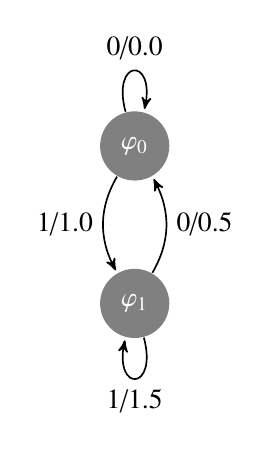
\begin{tikzpicture}[->,>=stealth',shorten >=1pt,auto,node distance=2.0cm,semithick]
  \tikzstyle{every state}=[fill=gray,draw=none,text=white]

  \node[state]         (B) {$\varphi_0$};

  \node[state]         (E) [below of=B]       {$\varphi_1$};

   \path     (B) edge [loop above] node {0/0.0} (B)
   			 (E) edge [bend right]  node[right] {0/0.5} (B)
             (B) edge[bend right]node[left]{1/1.0} (E)
        	 (E)  edge [loop below] node {1/1.5} (E);
\end{tikzpicture}

}
\caption{Finite state machine. }
\label{fig:FSM}
\end{figure}
The Trellis diagram for the FSM shown in Fig. \ref{fig:FSM} is given in Fig. \ref{fig:trellis}
\begin{figure}[h]
\centering
\resizebox{\columnwidth}{!}{
%\resizebox{\columnwidth}{!}{
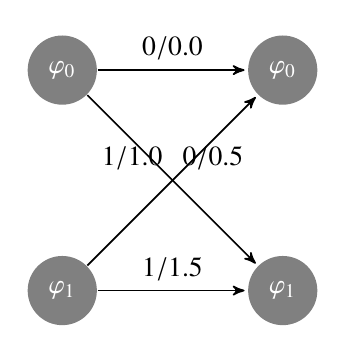
\begin{tikzpicture}[->,>=stealth',shorten >=1pt,auto,node distance=2.8cm,
                    semithick]
  \tikzstyle{every state}=[fill=gray,draw=none,text=white]

  \node[state] 			(A)                   {$\varphi_0$};
  \node[state]         (B) [ right of=A] {$\varphi_0$};
  \node[state]         (D) [below  of=A] {$\varphi_1$};
  \node[state]         (C) [below  of=B] {$\varphi_1$};
 
 
 \path (A) edge              node {$0/0.0$} (B)
            edge              node {$0/0.5$} (C)
        
            
        (D) edge              node {$1/1.5$} (C)
            
        
            edge              node {$1/1.0$} (B);
        


  
\end{tikzpicture}

}
\caption{Trellis Diagram. }
\label{fig:trellis}
\end{figure}

The multi-stage trellis diagram is shown in Fig. \ref{fig:multi-stage}.
\begin{figure}[h]
\centering
\resizebox{\columnwidth}{!}{
%\resizebox{\columnwidth}{!}{
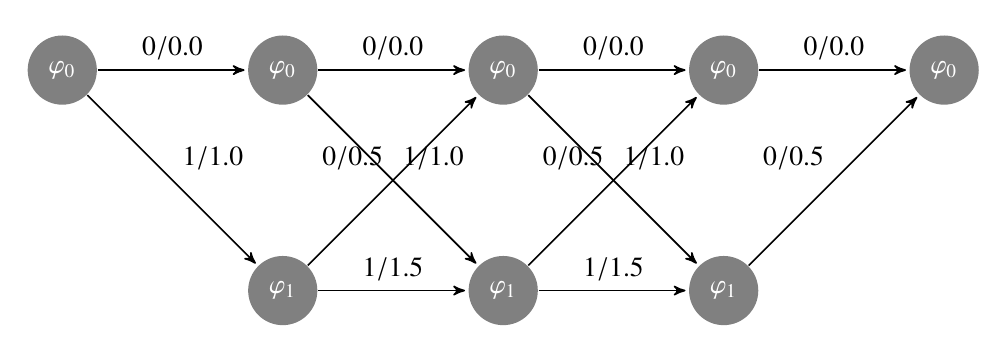
\begin{tikzpicture}[->,>=stealth',shorten >=1pt,auto,node distance=2.8cm,
                    semithick]
  \tikzstyle{every state}=[fill=gray,draw=none,text=white]

  \node[state] (A)                    {$\varphi_0$};
  \node[state]         (B) [right of=A] {$\varphi_0$};
  \node[state]         (C) [right of=B] {$\varphi_0$};
  \node[state]         (D) [right of=C] {$\varphi_0$};
  \node[state]         (E) [right of=D] {$\varphi_0$};
  \node[state]         (F) [below of=B] {$\varphi_1$};
  \node[state]         (G) [right of=F] {$\varphi_1$};    
  \node[state]         (H) [right of=G] {$\varphi_1$};   
  \path (A) edge              node {$0/0.0$} (B)
            edge              node {$1/1.0$} (F)
        (B) edge              node {$0/0.0$} (C)
            edge              node {$1/1.0$} (G)
        (C) edge              node {$0/0.0$} (D)
            edge              node {$1/1.0$} (H)
        (D) edge              node {$0/0.0$} (E)
        (F) edge              node {$0/0.5$} (C)
            edge              node {$1/1.5$} (G) 
        (G) edge              node {$0/0.5$} (D)
            edge              node {$1/1.5$} (H) 
        (H) edge              node {$0/0.5$} (E);
\end{tikzpicture}

}
\caption{Trellis Diagram. }
\label{fig:multi-stage}
\end{figure}

Suppose, we receive $r_k = [0.2,0.6,0.9,0.1]$ symbols at time instants $k=0,1,2,3$
\begin{itemize}
\item With Symbol-by-Symbol detection:
\begin{itemize}
\item Detection threshold  $= 0.5$.
\item Detected Symbols are $[0,1,1,0]$
\end{itemize}
\item ML detection/Minimum distance metric to be minimized
\begin{align}
\zeta_i = \sum_k \vert r_k - s_{k,i} \vert^2
\end{align}
Where, $i$ is over different transmit symbol vectors
\begin{equation}
\zeta_i = (r_0 - s_{0,i})^2 + (r_2 - s_{2,i})^2 \\ + (r_2 - s_{2,i})^2 + (r_3 - s_{3,i})^2
\label{eq:distance_metric}
\end{equation}
So, the branc metric at $k^{th}$ symbol period is
\begin{equation}
\zeta_{k,i} = (r_k - s_{k,i})^2
\end{equation}
Sum of these branch metrics to be minimized in MLSE.
\end{itemize}
The Trellis Diagram with branch metrics is shown in Fig. \ref{fig:branch_metric}.
\begin{figure}[h]
\centering
\resizebox{\columnwidth}{!}{
%\resizebox{\columnwidth}{!}{
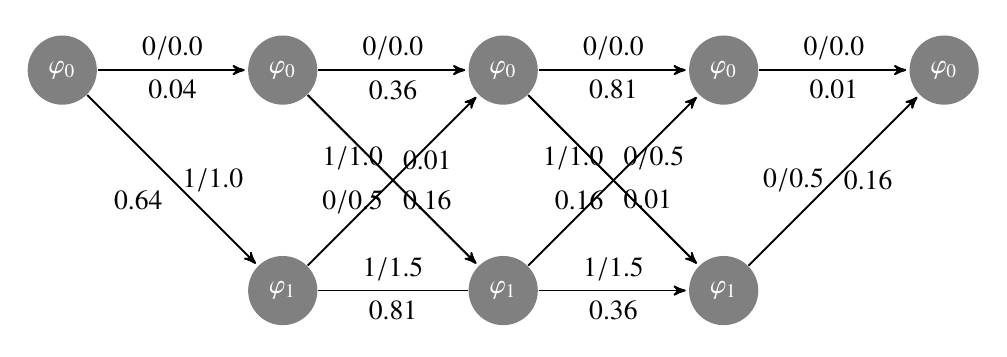
\begin{tikzpicture}[->,>=stealth',shorten >=1pt,auto,node distance=2.8cm,
                    semithick]
  \tikzstyle{every state}=[fill=gray,draw=none,text=white]

  \node[state] (A)                    {$\varphi_0$};
  \node[state]         (B) [right of=A] {$\varphi_0$};
  \node[state]         (C) [right of=B] {$\varphi_0$};
  \node[state]         (D) [right of=C] {$\varphi_0$};
  \node[state]         (E) [right of=D] {$\varphi_0$};
  \node[state]         (F) [below of=B] {$\varphi_1$};
  \node[state]         (G) [right of=F] {$\varphi_1$};    
  \node[state]         (H) [right of=G] {$\varphi_1$};   
  \draw (A)--node[above] {$0/0.0$}(B);
  \draw (A)--node[below] {$0.04$}(B);
  \draw (A)--node[right] {$1/1.0$}(F);
  \draw (A)--node[below left] {$0.64$}(F);
  \draw (B)--node[above] {$0/0.0$}(C);
  \draw (B)--node[below] {$0.36$}(C);
  \draw (C)--node[above] {$0/0.0$}(D);
  \draw (C)--node[below] {$0.81$}(D);
  \draw (D)--node[above] {$0/0.0$}(E);
  \draw (D)--node[below] {$0.01$}(E);
  \draw (B)--node[above left] {$1/1.0$}(G);
  \draw (B)--node[above right] {$0.01$}(G);
  \draw (F)--node[below left] {$0/0.5$}(C);
  \draw (F)--node[below right] {$0.16$}(C);
  \draw (C)--node[above left] {$1/1.0$}(H);
  \draw (C)--node[below right] {$0.01$}(H);
  \draw (G)--node[above right] {$0/0.5$}(D);
  \draw (G)--node[below left] {$0.16$}(D);
  \draw (H)--node[left] {$0/0.5$}(E);
  \draw (H)--node[right] {$0.16$}(E);
  \draw (F)--node[above] {$1/1.5$}(G) --node[above] {$1/1.5$}(H);
  \draw (F)--node[below] {$0.81$}(G) --node[below] {$0.36$}(H);
\end{tikzpicture}

}
\caption{Trellis Diagram with branch metrics. }
\label{fig:branch_metric}
\end{figure}
The shortest path using Viterbi Algorithm (VA) is shown in Fig. \ref{fig:shortest_path}.
\begin{figure}[h]
\centering
\resizebox{\columnwidth}{!}{
%\resizebox{\columnwidth}{!}{
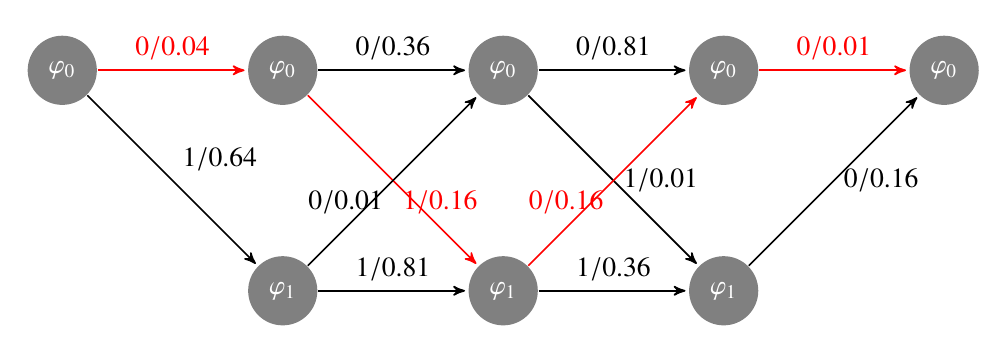
\begin{tikzpicture}[->,>=stealth',shorten >=1pt,auto,node distance=2.8cm,
                    semithick]
  \tikzstyle{every state}=[fill=gray,draw=none,text=white]

  \node[state] (A)                    {$\varphi_0$};
  \node[state]         (B) [right of=A] {$\varphi_0$};
  \node[state]         (C) [right of=B] {$\varphi_0$};
  \node[state]         (D) [right of=C] {$\varphi_0$};
  \node[state]         (E) [right of=D] {$\varphi_0$};
  \node[state]         (F) [below of=B] {$\varphi_1$};
  \node[state]         (G) [right of=F] {$\varphi_1$};    
  \node[state]         (H) [right of=G] {$\varphi_1$};   
  \path (A) edge [color=red]              node {$0/0.04$} (B)
            edge              node {$1/0.64$} (F)
        (B) edge              node {$0/0.36$} (C)
            edge [color=red]             node[below right] {$1/0.16$} (G)
        (C) edge              node {$0/0.81$} (D)
            edge              node[right] {$1/0.01$} (H)
        (D) edge [color=red]             node {$0/0.01$} (E)
        (F) edge               node[below left] {$0/0.01$} (C)
            edge              node {$1/0.81$} (G) 
        (G) edge[color=red]              node[below left] {$0/0.16$} (D)
            edge              node {$1/0.36$} (H) 
        (H) edge              node[right] {$0/0.16$} (E);
\end{tikzpicture}

}
\caption{Trellis Diagram with branch metrics. }
\label{fig:shortest_path}
\end{figure}
The symbol-by-symbol detection gives $[0,1,1,0]$ and
Maximum Likelihood sequence estimation (Via VA) gives $[0,1,0,0]$.
\subsubsection{Trellis structure in Code}
There are total $M^{L-1}$ states in the trellis. The complexity of viterbi algorithm increases with the length of the channel filter.
Suppose $L=3$ and number of states in trellis $64$. The total number of outpus from the trellis is
\begin{align}
trellis\_out\_size &= 64*M 
\end{align} 
$Trellis\_in\_struct$ and $Trellis\_out\_struct$ 

The ML sequence estimator structure using viterbi algorithm  \cite{viterbi} is shown in \cite{MLSE} and \cite{Proakis}.
To estimate a sequence of length $m$, the receiver complexity is $M^m$ symbols for finding the most likely sequence among $M^m$ sequences. However, this complexity can be reduced from $M^m$ to $M^{L-1}$, where $L$ is the number of states in trellis used for viterbi Algorithm ($L < m$).

The number of the states in the trellis increaes exponetially ($M^{L-1}$) with lenghth of the channel impulse response ($L$). Since the bandwidth requirement is $250$ Khz, the length of the impulse response is suficient to assume as $3$ and implemneted the viterbi algorithm with $64$ states.

\section{Channel Estimation}
The MLSE via Viterbi Algorithm needs the channel state information for finding the shortest path. The channel can be estimated using Fast Fourier transforms for a sequence of pilot symbols.

We have used $10$ pilot symbols in the code for the estimation of channel. The observed symbols at the receiver  for the pilot symbols is given by
\begin{equation}
\textbf{r}_{p} = \textbf{h}*\textbf{x}_{p} + \textbf{n}_{p}
\end{equation}

The steps for channel estimation is given below 
\begin{itemize}
\item Make $\textbf{r}_{p}$ into a circular convolution of \textbf{h} and $\textbf{x}_{p}$ by removing  last $L-1$ symbols from $\textbf{r}_{p}$ to add them to the first $L-1$ symbols .
\item Find 
\begin{align}
Y = fft \left(\textbf{r}_{p}\right) \quad X = fft \left(\textbf{x}_{p}\right) 
\end{align}
\item Find first three taps of $h_{est}$ from
\begin{align}
h_{est} = ifft\left(\frac{Y}{X}\right)
\end{align}
 \end{itemize}
 
The second method for channel estimation based on Toeplitz matrix method with pilot symbols is given below
\begin{itemize}
\item Construct a toeplitz matrix $X$  with pilot symbols $x_p$.
\item 
\begin{align}
h_est = \left(X^{*}X\right)^{-1}X^{*}y_p
\end{align}
\end{itemize}

\section{Zero Forcing Equalizer and MMSE Equalizer}
The Zero-Forcing Equalizer and MMSE are implemente using Toeplitz matrices \cite{eq}.
\subsection{Zero Forcing Equalizer}
\begin{itemize}
\item Construct a toeplitz matrix $H$  with estimated channel $h_{est}$.
\item 
\begin{align}
x_{hat} = \left(H^{*}H\right)^{-1}H^{*}y
\end{align}
\end{itemize}
\subsection{MMSE Equalizer}
\begin{itemize}
\item Construct a toeplitz matrix $H$  with estimated channel $h_{est}$.
\item 
\begin{align}
x_{hat} = \left(H^{*}H + \frac{I}{SNR} \right)^{-1}H^{*}y
\end{align}
Where, $I$ is an identity matrix and $SNR$ is the signal-to-noise ratio.
\end{itemize}

%\section{Simulation results}
%We have trained for $100$ $8-PSK$ symbols ($30$ Frames ($1 Frame = 40 bytes$)) for $15$ iterations and in Fig.\ref{fig:MMSE} and Fig. \ref{fig:DFE}, the convergence of cost function (Mean Square Error (MSE)) w.r.to the number of iterations for both MMSE and DFE equalizers are shown.
%%\subsection{Plots}
%\begin{figure}[t]
%\begin{center}
%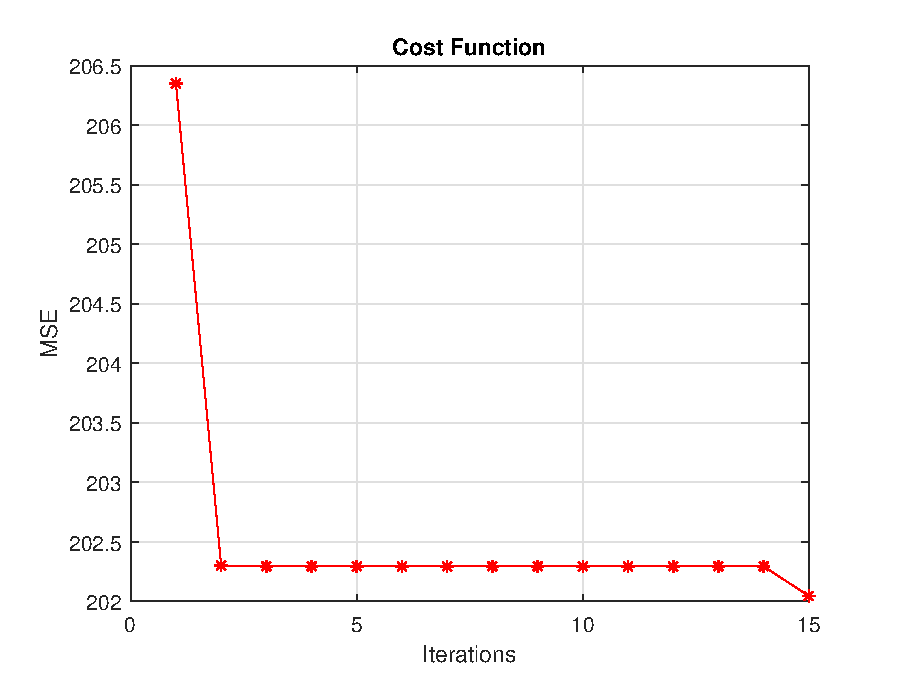
\includegraphics[width=\columnwidth]{./figs/Cost Function MMSE.eps}
%\end{center}
%\caption{Mean Sqaure Error Vs Iterations for MMSE}
%\label{fig:MMSE}
%\end{figure}
%
%\begin{figure}[t]
%\begin{center}
%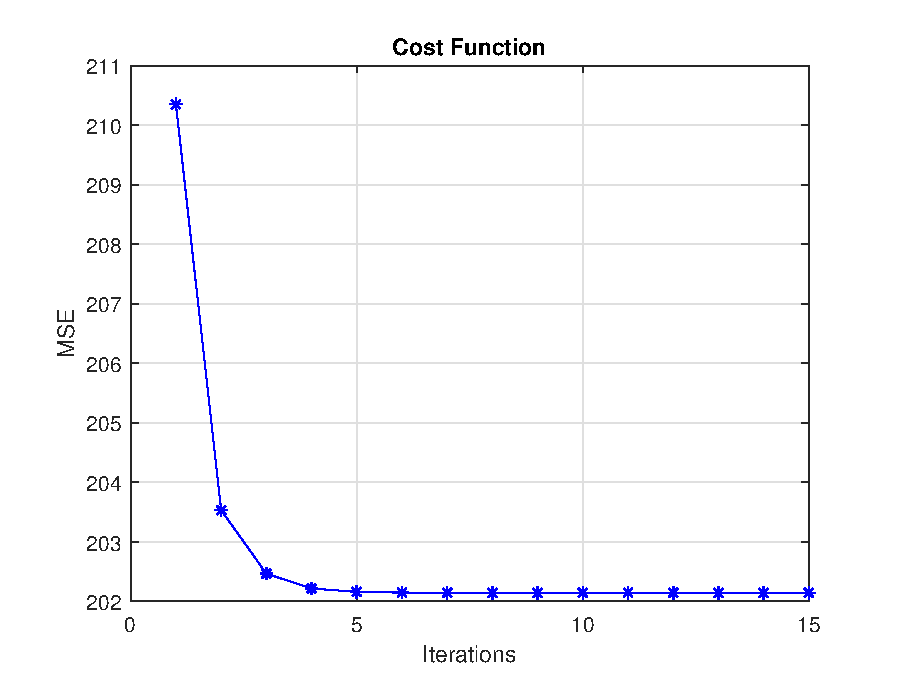
\includegraphics[width=\columnwidth]{./figs/Cost Function DFE.eps}
%\end{center}
%\caption{Mean Sqaure Error Vs Iterations for MMSE}
%\label{fig:DFE}
%\end{figure}
%
%Table \ref{table:comparisions} compares the different equalizers explained in previous sections.
%
%\begin{table}[b]
%\caption{Comparision of different Equalizers}
%\begin{center}
%\begin{tabular}{|c|c|c|c|}
%\hline
%\textbf{Equalizer}& \textbf{Frames} & \text{Time} & \textbf{Complexity}\\
%    \hline
%    $MMSE$ & 60 & 120 ms & Medium\\ %\quad \cite{bitnodes} \\
%    \hline
%    $DFE$ & 120 & 240 ms & Medium\\ %\quad \cite{bitnodes}  \\
%    \hline
%    $MLSE$ & $-$ & $-$ & High \\
%		\hline
%	
%\end{tabular}
%\label{table:comparisions}
%\end{center}
%\end{table}
%
%
%Fig.\ref{fig:ser} shows the SER curve ($\frac{E_b}{N_0} vs P_{e}$).
%\begin{figure}[!t]
%\begin{center}
%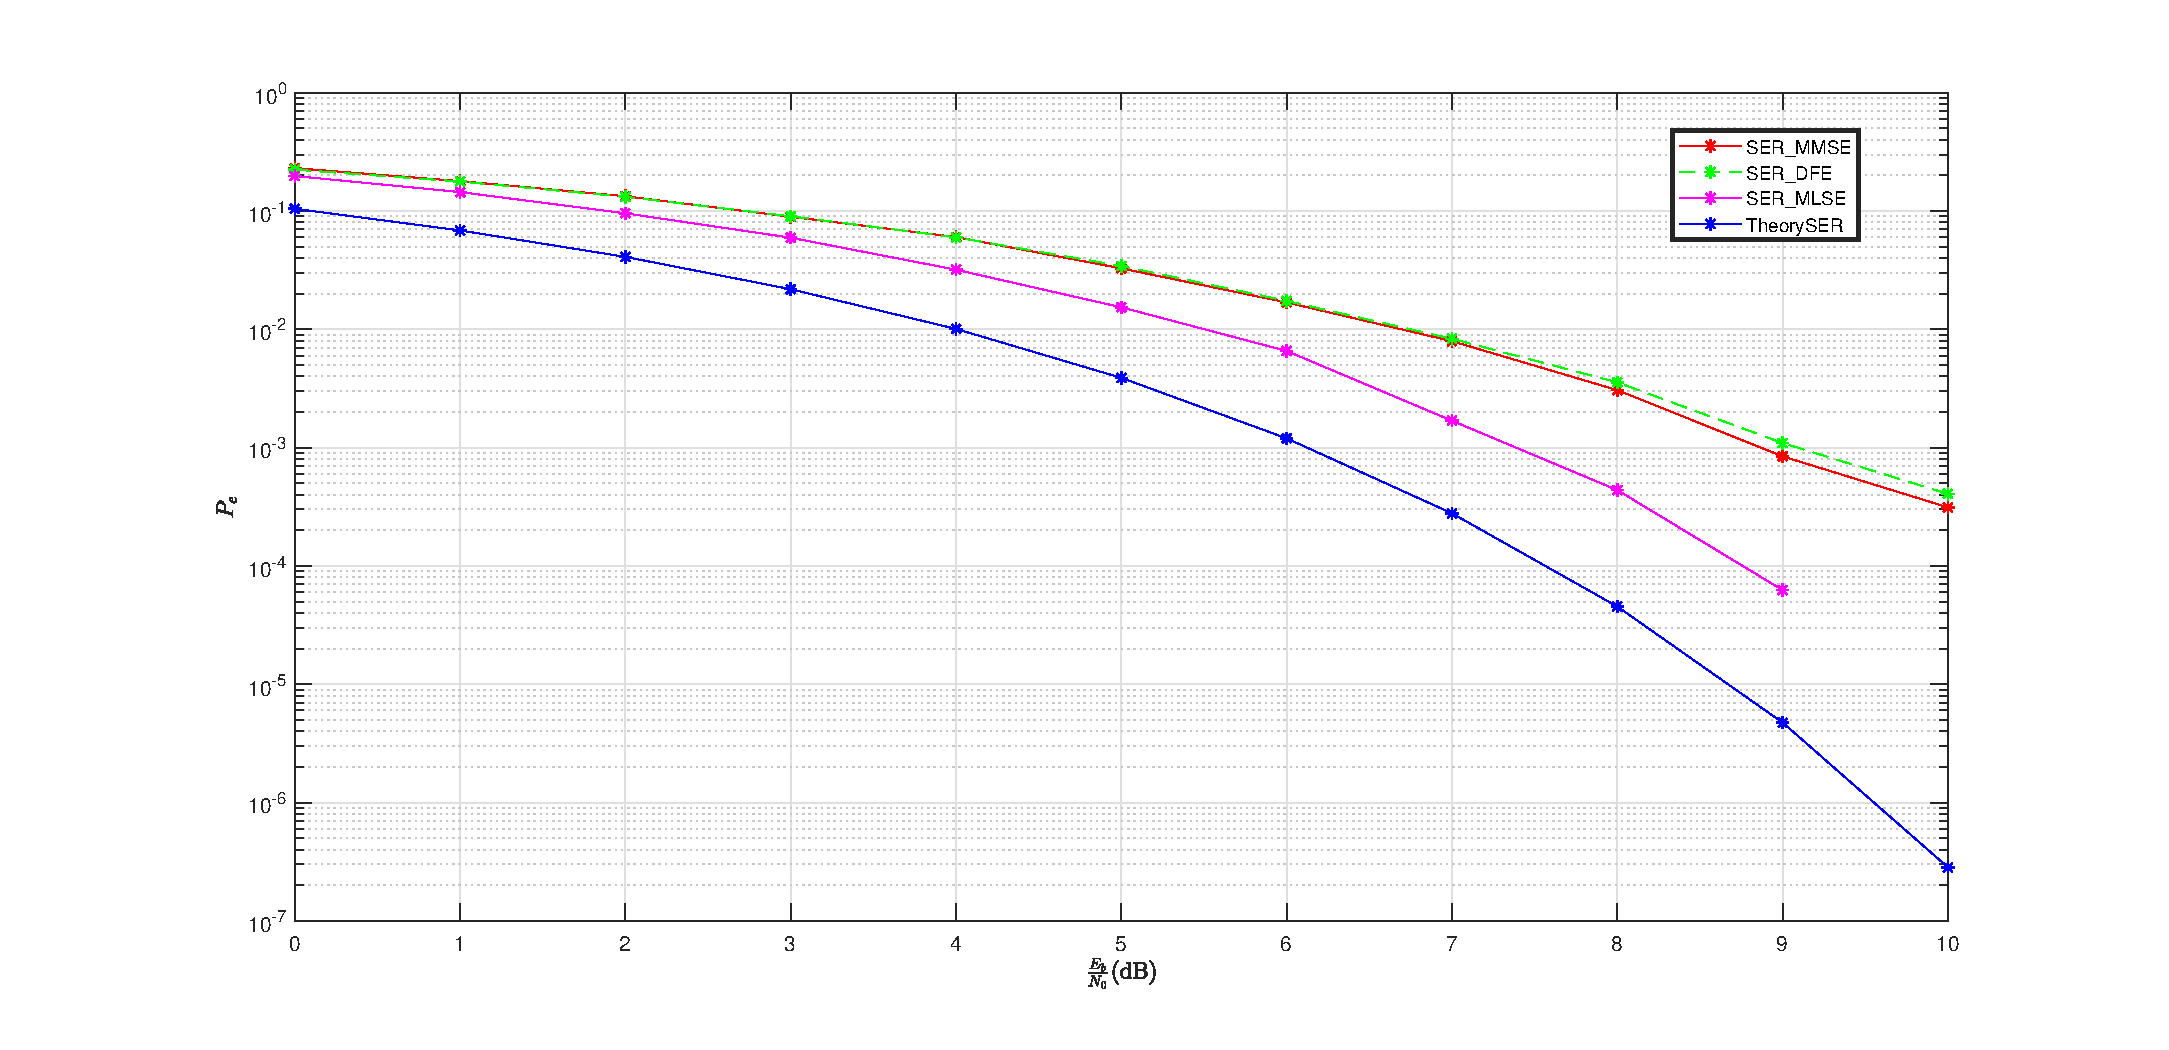
\includegraphics[width=\columnwidth]{./figs/Equalizers_1.eps}
%\end{center}
%\caption{Symbol Error Rate}
%\label{fig:ser}
%\end{figure}
%
%
\bibliography{IEEEabrv,equalizer_design}
%\bibliography{IEEEabrv,equalization.bib}
\end{document}


